\documentclass[border=2pt]{standalone}
% Shared style for the vector figures (Figs. 1, 2, 4). Compile each fig*.tex with pdflatex.
\usepackage[T1]{fontenc}
\usepackage{lmodern}
\usepackage{amsmath,amssymb}
\usepackage{sansmath}
\usepackage{tikz}
\usetikzlibrary{arrows.meta,calc,positioning,fit,patterns,decorations.pathreplacing}
\renewcommand{\familydefault}{\sfdefault}
\sansmath
% class colours (blue, green, orange, purple, grey): distinguishable in greyscale by label, not by colour alone
\definecolor{cD}{HTML}{1F5FAE}
\definecolor{cL}{HTML}{1B7F4B}
\definecolor{cP}{HTML}{C2590F}
\definecolor{cG}{HTML}{6A3D9A}
\definecolor{cH}{HTML}{4D4D4D}
\definecolor{cA}{HTML}{8A5A00}   % PPA (event audit)
\definecolor{ink}{HTML}{1A1A1A}
\definecolor{rule}{HTML}{8C8C8C}
\tikzset{
  >={Stealth[length=5pt,width=4pt]},
  every picture/.style={line cap=round,line join=round,text=ink},
  box/.style={draw=#1,line width=0.7pt,rounded corners=2.5pt,fill=#1!7,align=center,inner sep=3pt},
  plain/.style={draw=rule,line width=0.6pt,rounded corners=2.5pt,fill=white,align=center,inner sep=3pt},
  flow/.style={->,line width=0.6pt,draw=ink!85},
}
\hyphenpenalty=10000\exhyphenpenalty=10000

\begin{document}
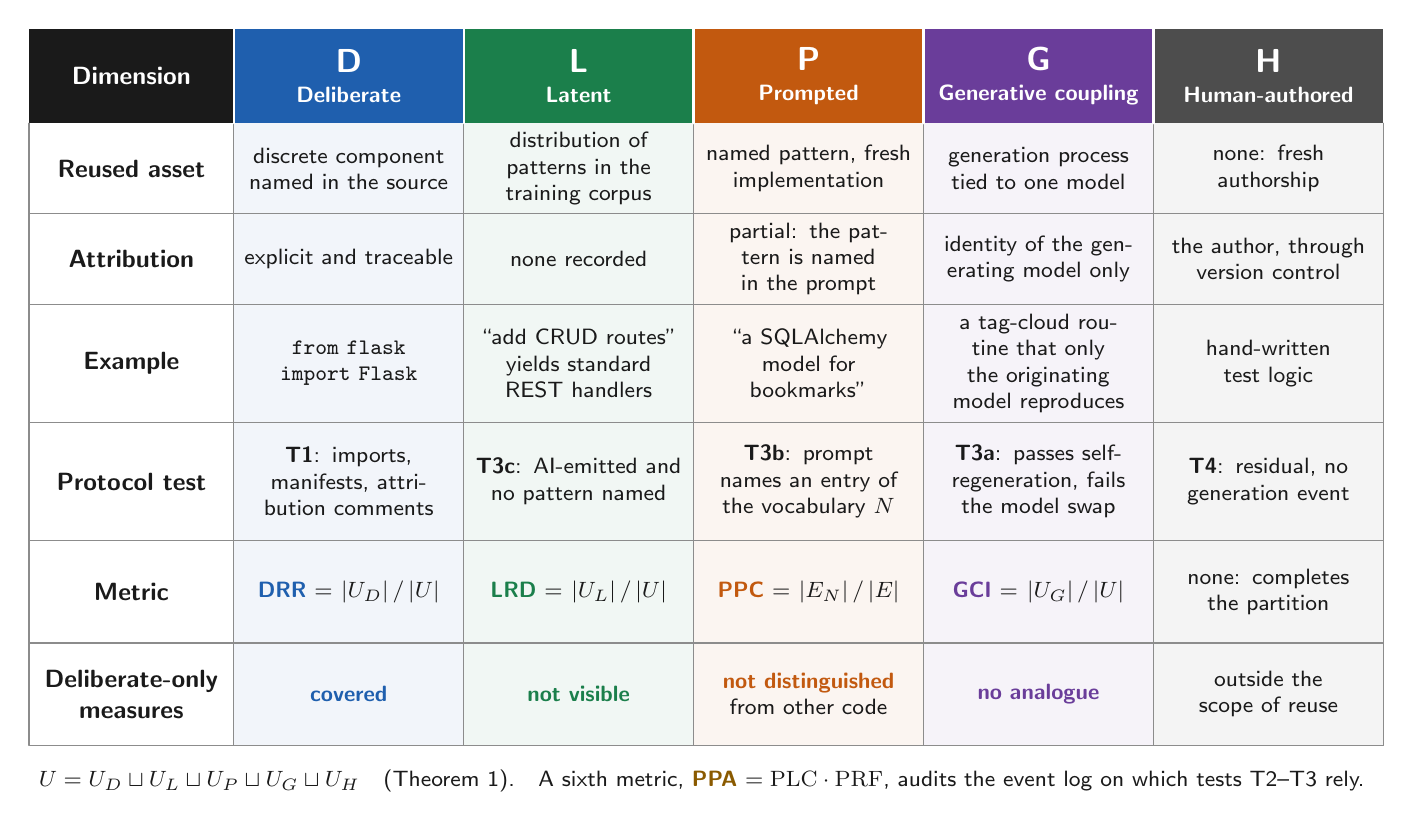
\begin{tikzpicture}[x=1cm,y=1cm]
% geometry: header column 2.3 wide, five class columns 2.98 wide -> 17.2 total
\def\hw{2.6}\def\cw{2.92}\def\hh{1.2}
\newcommand{\colx}[1]{\hw+#1*\cw-0.5*\cw}
% row tops (y) and heights: header, asset, attribution, example, test, metric, coverage
% ---------------- header row
\foreach \i/\c/\l/\n in {1/cD/D/Deliberate,2/cL/L/Latent,3/cP/P/Prompted,4/cG/G/Generative coupling,5/cH/H/Human-authored}{
  \fill[\c] ({\hw+(\i-1)*\cw},0) rectangle ({\hw+\i*\cw},-\hh);
  \node[text=white,align=center] at ({\colx{\i}},-0.5*\hh) {{\large\bfseries \l}\\[-1pt]{\footnotesize\bfseries \n}};
  % tinted column body
  \fill[\c!6] ({\hw+(\i-1)*\cw},-\hh) rectangle ({\hw+\i*\cw},-9.1);
}
\fill[ink] (0,0) rectangle (\hw,-\hh);
\node[text=white,font=\small\bfseries] at (0.5*\hw,-0.5*\hh) {Dimension};
% ---------------- rows
\newcommand{\row}[8]{% ytop, height, label, D, L, P, G, H
  \pgfmathsetmacro{\ym}{#1-0.5*#2}
  \node[font=\small\bfseries,align=center,text width=2.4cm] at (0.5*\hw,\ym) {#3};
  \node[font=\footnotesize,align=center,text width=2.66cm] at ({\colx{1}},\ym) {#4};
  \node[font=\footnotesize,align=center,text width=2.66cm] at ({\colx{2}},\ym) {#5};
  \node[font=\footnotesize,align=center,text width=2.66cm] at ({\colx{3}},\ym) {#6};
  \node[font=\footnotesize,align=center,text width=2.66cm] at ({\colx{4}},\ym) {#7};
  \node[font=\footnotesize,align=center,text width=2.66cm] at ({\colx{5}},\ym) {#8};
  \draw[rule,line width=0.4pt] (0,#1-#2) -- (17.2,#1-#2);}
\row{-1.2}{1.15}{Reused asset}
  {discrete component named in the source}
  {distribution of patterns in the training corpus}
  {named pattern, fresh implementation}
  {generation process tied to one model}
  {none: fresh authorship}
\row{-2.35}{1.15}{Attribution}
  {explicit and traceable}
  {none recorded}
  {partial: the pattern is named in the prompt}
  {identity of the generating model only}
  {the author, through version control}
\row{-3.5}{1.5}{Example}
  {\texttt{from flask import Flask}}
  {``add CRUD routes'' yields standard REST handlers}
  {``a SQLAlchemy model for bookmarks''}
  {a tag-cloud routine that only the originating model reproduces}
  {hand-written test logic}
\row{-5.0}{1.5}{Protocol test}
  {\textbf{T1}: imports, manifests, attribution comments}
  {\textbf{T3c}: AI-emitted and no pattern named}
  {\textbf{T3b}: prompt names an entry of the vocabulary $N$}
  {\textbf{T3a}: passes self-regeneration, fails the model swap}
  {\textbf{T4}: residual, no generation event}
\row{-6.5}{1.3}{Metric}
  {{\color{cD}\textbf{DRR}} $= |U_D|\,/\,|U|$}
  {{\color{cL}\textbf{LRD}} $= |U_L|\,/\,|U|$}
  {{\color{cP}\textbf{PPC}} $= |E_N|\,/\,|E|$}
  {{\color{cG}\textbf{GCI}} $= |U_G|\,/\,|U|$}
  {none: completes the partition}
\row{-7.8}{1.3}{Deliberate-only measures}
  {{\color{cD}\textbf{covered}}}
  {{\color{cL}\textbf{not visible}}}
  {{\color{cP}\textbf{not distinguished}} from other code}
  {{\color{cG}\textbf{no analogue}}}
  {outside the scope of reuse}
% ---------------- grid
\foreach \i in {0,...,5} \draw[rule,line width=0.4pt] ({\hw+\i*\cw},-\hh) -- ({\hw+\i*\cw},-9.1);
\draw[rule,line width=0.4pt] (0,-\hh) -- (0,-9.1);
\foreach \i in {1,...,4} \draw[white,line width=0.8pt] ({\hw+\i*\cw},0) -- ({\hw+\i*\cw},-\hh);
\draw[white,line width=0.8pt] (\hw,0) -- (\hw,-\hh);
% ---------------- footer
\node[font=\footnotesize,anchor=west] at (0,-9.55)
  {$U = U_D \sqcup U_L \sqcup U_P \sqcup U_G \sqcup U_H$\quad (Theorem 1).\quad A sixth metric, {\color{cA}\textbf{PPA}} $= \mathrm{PLC}\cdot\mathrm{PRF}$, audits the event log on which tests T2--T3 rely.};
\end{tikzpicture}
\end{document}
